\newpage
\datos{color}{}{}
\section*{Desarrollo de la propuesta técnica de búsqueda evolutiva}
\addcontentsline{toc}{section}{Desarrollo de la propuesta técnica de búsqueda evolutiva}
En esta sección se resuelve el problema mediante la técnica evolutiva elegida 
en la propuesta del apartado anterior y se exponen los resultados obtenidos.\\

Se ha realizado un análisis de sensibilidad de \textit{Kruskal-Wallis} con el 
objetivo de estudiar la sensibilidad de los parámetros ($F$, $CR$) propios del 
algoritmo de evolución diferencial.

\subsection*{Resultados principales}
\addcontentsline{toc}{subsection}{Resultados principales}
Los resultados de la \autoref{tab:tema3_tabla2} muestran que el algoritmo presenta un comportamiento
estable y consistente a lo largo de las 30 ejecuciones realizadas. Además, ha obtenido mejores 
resultados que el algoritmo de búsqueda local (\autoref{tab:tema2_tabla2}), valores que se incluyen 
en la \autoref{tab:tema3_tabla2} para realizar la comparativa. \\

El valor medio de $T_{\max}$ es
de 1.31\,s, con una desviación típica moderada (0.23\,s), lo que indica que la variabilidad entre
ejecuciones es aún más baja que en el tema anterior. Esto es un indicador de que el algoritmo ha
sido más eficaz a la hora encontrar cuál es el espacio de modificaciones en el vector de soluciones para 
satisfacer en mayor grado a la función objetivo. El mejor caso alcanza un tiempo de 0.86\,s, mientras que el peor
se sitúa en 1.67\,s, lo que define el rango completo de rendimiento del método. El intervalo de 
confianza al 95\,\%, $[1.23,\,1.39]$\,s, confirma que, con alta probabilidad, el algoritmo converge
de forma consistente en torno a valores próximos a la media. \\

Por otro lado, el tiempo medio de ejecución del proceso completo es de 1.98\,s, lo que demuestra
que el método, aunque más costoso, sigue siendo computacionalmente eficiente y adecuado para
escenarios donde se requiere optimización rápida. A pesar de ese mayor coste, la mejora en 
los resultados lo compensa.\\

De forma complementaria, el diagrama de cajas de la \autoref{fig:cajaT_tema3} 
muestra que la mayor parte de las soluciones de $T_{\max}$ se concentran en un intervalo 
relativamente estrecho. El rango intercuartílico se sitúa aproximadamente entre 1.18\,s y 1.49\,s, 
lo que indica que el 50\% central de las ejecuciones produce soluciones de calidad similar.
El bigote inferior desciende hasta aproximadamente 0.85\,s, mientras que el superior alcanza
valores cercanos a 1.75\,s, lo que refleja la presencia de ejecuciones tanto muy
buenas como menos favorables. No obstante, la ausencia de valores atípicos sugiere que
estas variaciones se encuentran dentro del comportamiento esperado del método.

%En conjunto, el diagrama evidencia que el algoritmo es estable, con una dispersión moderada y sin
%comportamientos anómalos.

\begin{table}[H]
\centering
\begin{tabular}{|l|c|c|c|}
\hline
\textbf{Métrica} & \cellcolor{yellow!30}\textbf{Valor} & \textbf{Valor anterior (tema 2)} & \textbf{Diferencia} \\
\hline
Media de $T_{\max}$ & \cellcolor{yellow!30}1.31 s & 1.67 & -21.6\% \\
Desviación típica & \cellcolor{yellow!30}0.23 & 0.50 & -54.0\% \\
Mejor valor (mínimo) & \cellcolor{yellow!30}0.86 s & 0.96 & -10.4\% \\
Peor valor (máximo) & \cellcolor{yellow!30}1.67 s & 2.88 & -42.0\% \\
Intervalo de confianza 95\% & \cellcolor{yellow!30}[1.23, 1.39] s & [1.49, 1.88] & -17.4\% \\ 
Tiempo medio de ejecución (s) & \cellcolor{yellow!30}1.98 s & 0.83 & +138.6\% \\
\hline
\end{tabular}
\caption{Métricas agregadas calculadas sobre las 30 ejecuciones de evolución diferencial.}
\label{tab:tema3_tabla2}
\end{table}

\begin{figure}[H]
  \centering
  
\includegraphics[scale=0.27]{Images/tema3/boxplot_Tmax.png}
  \caption{Diagrama de caja de la solución temporal evolutiva.}
  \label{fig:cajaT_tema3}
\end{figure}

También resulta interesante evaluar la variabilidad en los puntos espaciales explorados. En 
la \autoref{fig:cajaP_tema3} se presenta el diagrama de caja para la coordenada $x$ de los puntos A 
y B. La mayoría de las soluciones se agrupan en el intervalo $[0.2, 0.4]$ metros y $[0.4, 0.6]$
metros, lo que
induce a pensar que esas zonas son las regiones más estables, alcanzables o cinemáticamente factibles
para los robots. En la \autoref{fig:visP_tema3} se visualizan en tres dimensiones los 30 puntos explorados.

\begin{figure}[H]
  \centering
  
\includegraphics[scale=0.24]{Images/tema3/boxplot_pA_x_pB_x.png}
  \caption{Diagrama de caja del punto espacial en el tema 3.}
  \label{fig:cajaP_tema3}
\end{figure}
\begin{figure}[H]
  \centering
  
\includegraphics[scale=0.15]{Images/tema3/visualizacion_pA_pB.png}
  \caption{Visualización de los puntos espaciales factibles optimizados en el tema 3.}
  \label{fig:visP_tema3}
\end{figure}
En la \autoref{fig:curvaMedia} se presenta la curva de convergencia del método, 
donde se observa que el algoritmo ha convergido a las 3 generaciones de las 150 que se realizan.
Este resultado llamativo, aparentemente conduce a pensar en la convergencia prematura del método.
Sin embargo, 

En la \autoref{fig:curvaMedia} se presenta la curva de convergencia del método, donde se observa
que el algoritmo ha convergido a las 3 generaciones de las 150 que se realizan. Este resultado,
aunque llamativo, no implica necesariamente una convergencia prematura. En realidad, es coherente
con la naturaleza del problema: en esta fase, el espacio efectivo del vector de decisión se 
reduce a un hipercubo de únicamente cuatro dimensiones (posición del raíl y tres factores de 
velocidad). En un dominio tan compacto, la evolución diferencial es capaz de desplazarse con 
gran rapidez hacia regiones prometedoras, estabilizando el valor de la función objetivo en 
muy pocas generaciones. \\

Además, los resultados obtenidos en la tabla muestran valores consistentes y estables entre 
ejecuciones, lo que indica que el algoritmo no solo converge rápido, sino que realiza una 
búsqueda ágil y de calidad, identificando de forma fiable zonas factibles y de buen rendimiento.
La ausencia de mejoras posteriores no se debe a estancamiento, sino a que el paisaje del 
problema —dominado por restricciones geométricas y cinemáticas muy estructuradas— ofrece pocas
oportunidades adicionales de optimización una vez alcanzada la región óptima. \\

Es importante justificar el uso de $J$ para graficar esta curva, ya que aunque la función de mérito utilizada en el nivel 2 del Temple 
Simulado se reduce a la
penalización de sincronización $J = P_{\text{sync}}(\Delta t), \qquad \Delta t = |t_A - t_B|,$
esta magnitud actúa como un mecanismo indirecto de minimización del tiempo dentro del punto
espacial seleccionado en el nivel 1, que sería la función objetivo. \\

Para que la penalización sea mínima, el algoritmo debe
ajustar los factores de velocidad y la posición del raíl de modo que ambos robots alcancen el
punto de cooperación en el mismo instante. Esta coincidencia temporal solo puede lograrse si
los tiempos individuales se igualan en el menor valor posible compatible con la geometría del
punto. En consecuencia, aunque el nivel 2 no modifica la posición espacial (que determina el
tiempo mínimo alcanzable), sí minimiza el tiempo de ejecución dentro de ese punto al
forzar la sincronización. \\

Por este motivo, las curvas de convergencia representan la evolución
de la función de mérito $J$, que es la magnitud que realmente guía el proceso de optimización.

\begin{figure}[H]
  \centering
  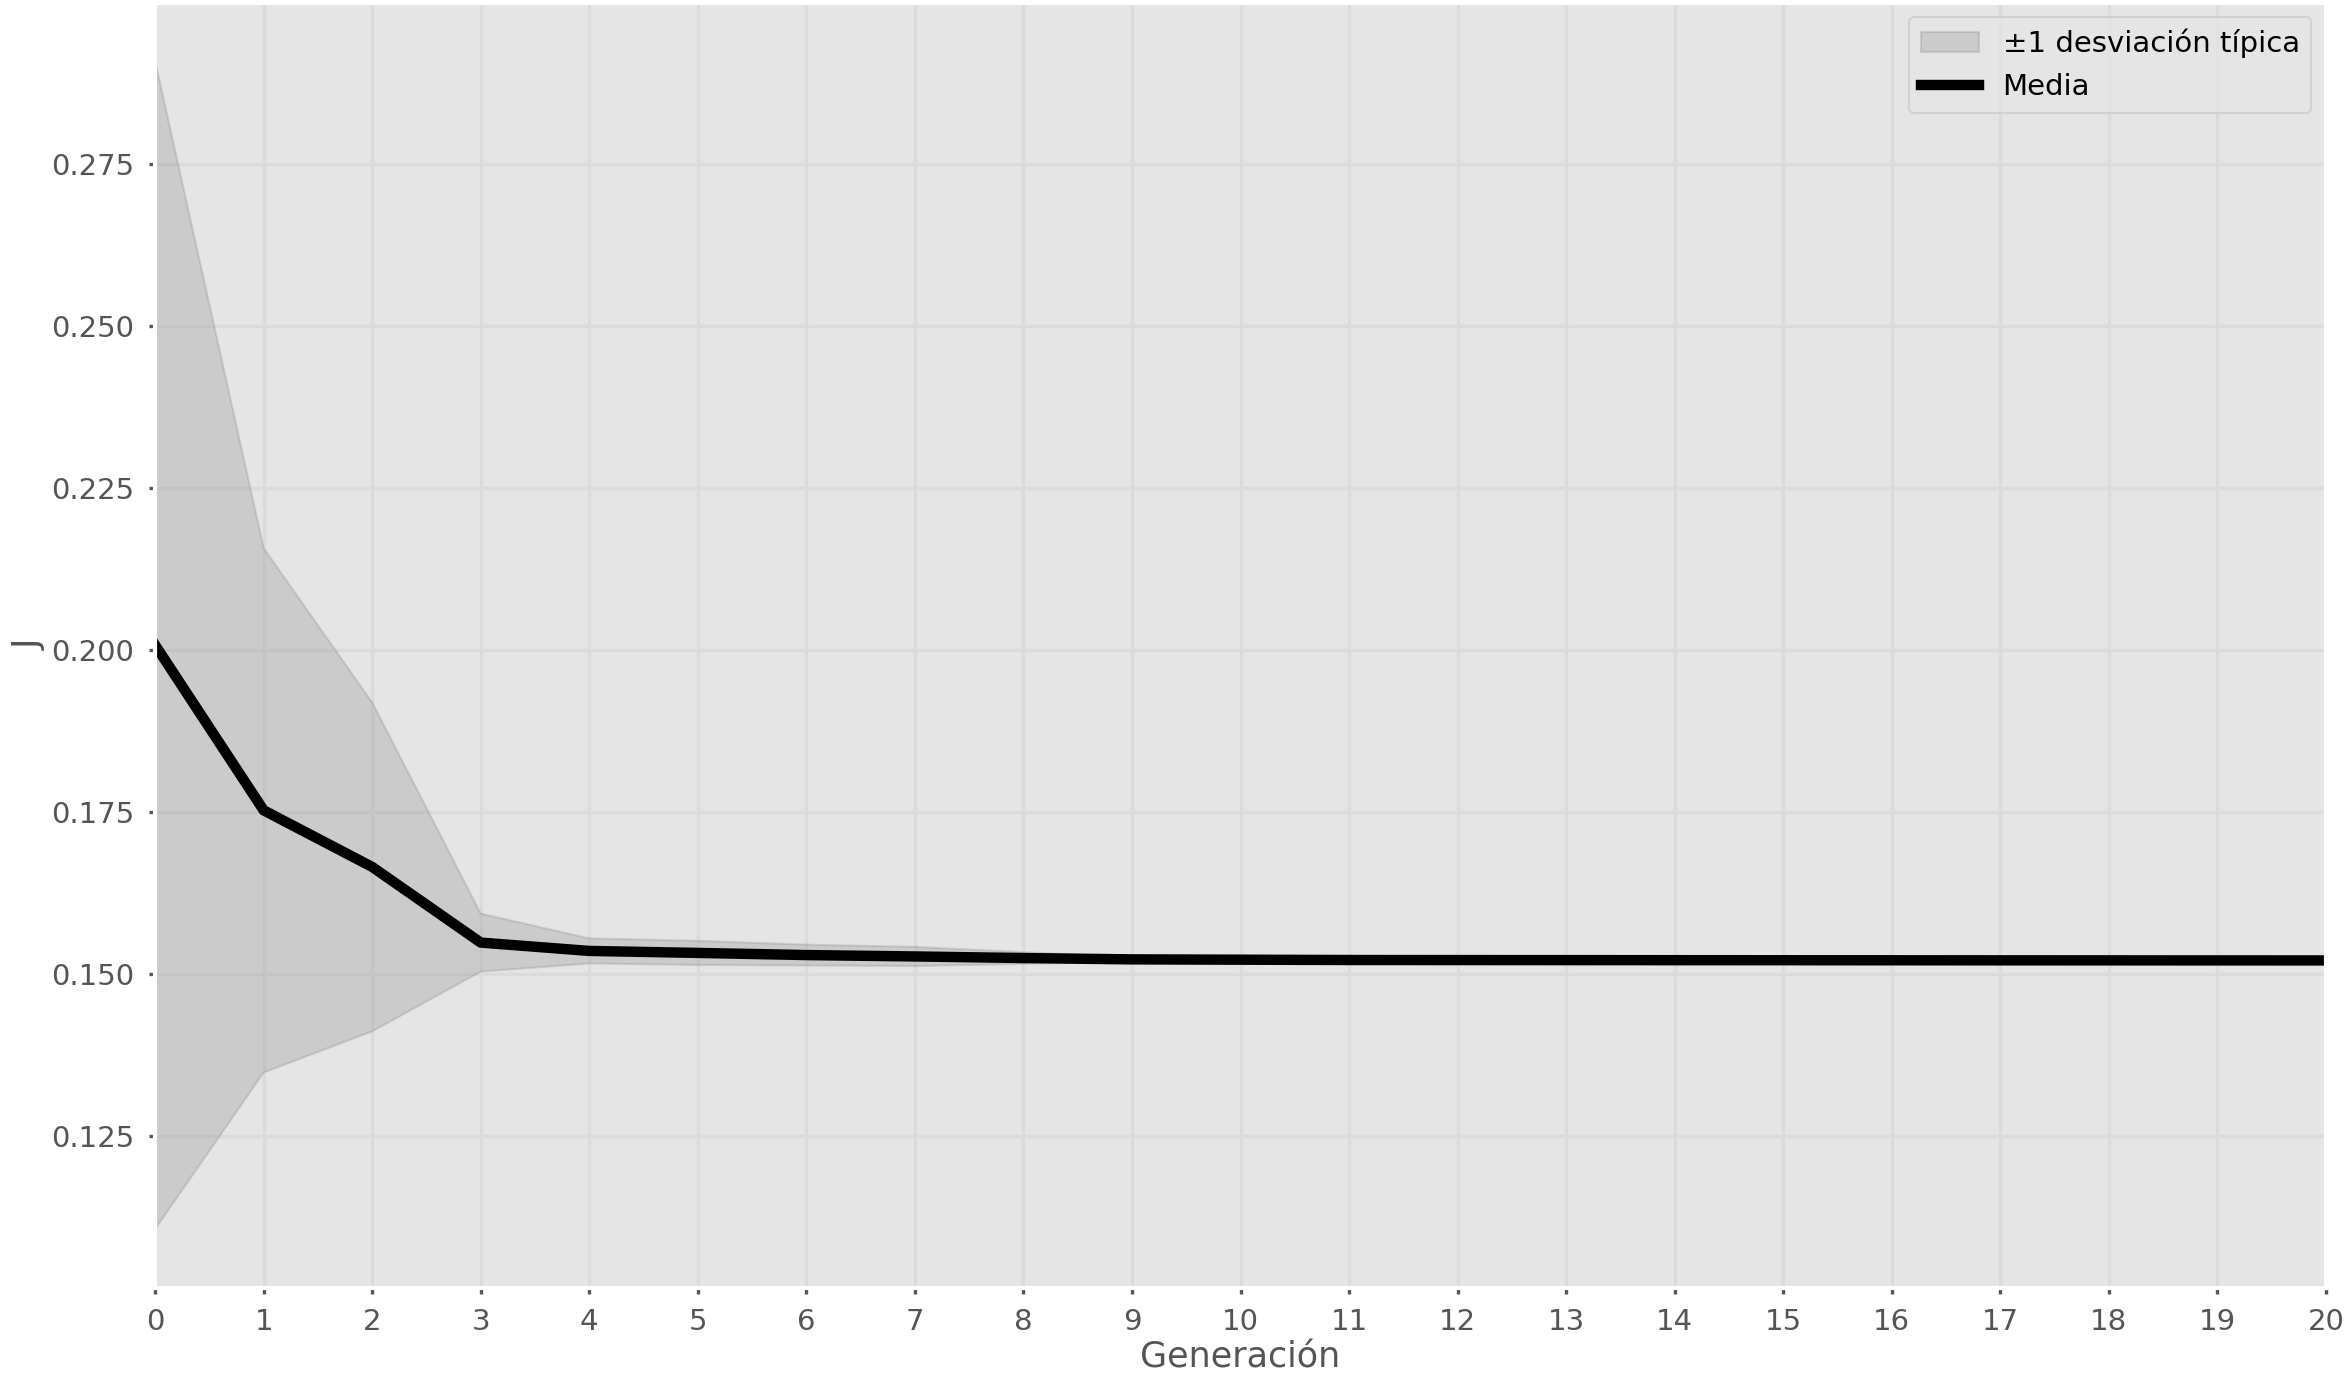
\includegraphics[scale=0.17]{Images/tema3/convergencia_J_media.png}
  \caption{Curva media de convergecia de la evolución diferencial, donde se aprecia la disminución
  de la penalización J.}
  \label{fig:curvaMedia}
\end{figure}


%En conjunto, estas métricas cuantitativas permiten concluir que el algoritmo no solo es eficaz
%en términos de calidad de las soluciones (medida mediante $T_{\max}$), sino también robusto y 
%estable en su comportamiento estadístico.


\subsection*{Conclusiones}
\addcontentsline{toc}{subsection}{Conclusiones}
Durante la evaluación de los resultados se ha observado que el algoritmo tiende a converger de forma
prematura, lo que sugiere que no está explorando completamente el espacio de soluciones
disponible. Sin embargo, las soluciones proporcionadas son muy lógicas, salvo por los perfiles 
de velocidad cuando estos reciben el máximo valor posible (1). \\

Resulta evidente que la mejor solución, es decir, aquella con menor tiempo de desplazamiento,
se obtiene con la máxima velocidad de los robots. Esta situación está introduciendo un sesgo al 
algoritmo para explorar únicamente perfiles elevados de velocidad, reduciendo el espacio de búsqueda, provocando una convergecia prematura y priorizando la minimización del tiempo a costa de ignorar
criterios de calidad del movimiento que serían relevantes en un escenario real. \\

Así todo, no todos los perfiles de velocidad optimizados son elevados, puesto que 
en la mejor solución obtenida la escala de velocidad del robot A es de $0.41$. 
Consecuentemente, demuestra que a pesar de que el algoritmo tenga un sesgo, es capaz 
de optimizar parcialmente el punto de encuentro de ambos robots. \\

La eliminación de este sesgo se plantea como línea futura, mediante la introducción
de alguna restricción sobre aceleración, suavidad o calidad de movimiento. \\

Además, el método implementado es computacionalmente eficiente puesto que 
los tiempos de ejecución son muy bajos, pudiendo ser utilizado en apliaciones de planificación 
de trayectorias de robots. \\

Por úlitmo, otro trabajo futuro que se plantea es la resolución del problema con la metodología
mencionada previamente: establecer un mecanismo de evaluación que determine cómo de lejos se 
encuentra un punto del espacio de trabajo factible para que el algoritmo de 
Temple Simulado sea capaz de converger hacia puntos factibles.